\begin{frontmatter}

    \title{Comparative analysis of PMV Models accuracy implemented in the ISO 7730:2005 and ASHRAE 55:2023}

    \author[label1]{Federico Tartarini\corref{mycorrespondingauthor}}
    \ead{federico.tartarini@sydney.edu.au}
    \author[label3]{Stefano Schiavon}

    \address[label1]{School of Architecture, Design, and Planning, The University of Sydney, Sydney, AU}
    \address[label3]{Center for the Built Environment, Department of Architecture, Department of Civil and Environmental Engineering, University of California, Berkeley, CA, USA}

    \cortext[mycorrespondingauthor]{Corresponding author}

    \begin{abstract}
        The \ac{pmv} model, developed by Fanger, is still currently used in its original form in the \gls{7730}.
        It has a low prediction accuracy, especially outside thermal neutrality.
        Several other formulations have been proposed to compensate for its limitations.
        One is the \ac{pmv-ce} standard.
        The \gls{7730} and \gls{55} are the most widely referenced thermal comfort standards worldwide, and their different \ac{pmv} formulations are a source of confusion.
        Which model is more accurate?

        We compared the accuracy of the two \ac{pmv} formulations, against \var{entries_db_used} thermal sensation votes collected in buildings.
        We found that both models have low and similar prediction accuracy (\qty{34}{\percent}) and the \ac{pmv-ce} has higher bias than \ac{pmv} in predicting thermal sensation in the subset of data with \ac{v}~$\geq$~\qty{0.2}{\m\per\s}.
        We suggest reducing the applicability limit of the models within the range $\mid$\ac{pmv}$\mid \leq 0.5$ since the \ac{pmv} models cannot determine the degree to which people are dissatisfied.
        Both models have an accuracy lower or equal to \qty{7}{\percent} when predicting either `warm', `hot', or `cold'.
        This value is lower than random guessing (\qty{14}{\percent}), meaning they are misleading the users.
        A \ac{pmv} value higher than \num{.5} or lower than \num{-.5} only indicates that people's thermal sensation is on the `warm' or `cold' side, respectively.
        Finally, the assumption that individuals who feel `slightly warm' or `slightly cool' can be considered thermally neutral leads to under-counting thermal discomfort, therefore, we recommend using the thermal preference scale instead of the thermal sensation scale.
        In the \ac{db2} \qty{68}{\percent} of participants who were `slightly warm' wanted to be `cooler' and \qty{54}{\percent} of participants who were `slightly cool' wanted to be `warmer'.
    \end{abstract}

    \begin{graphicalabstract}
        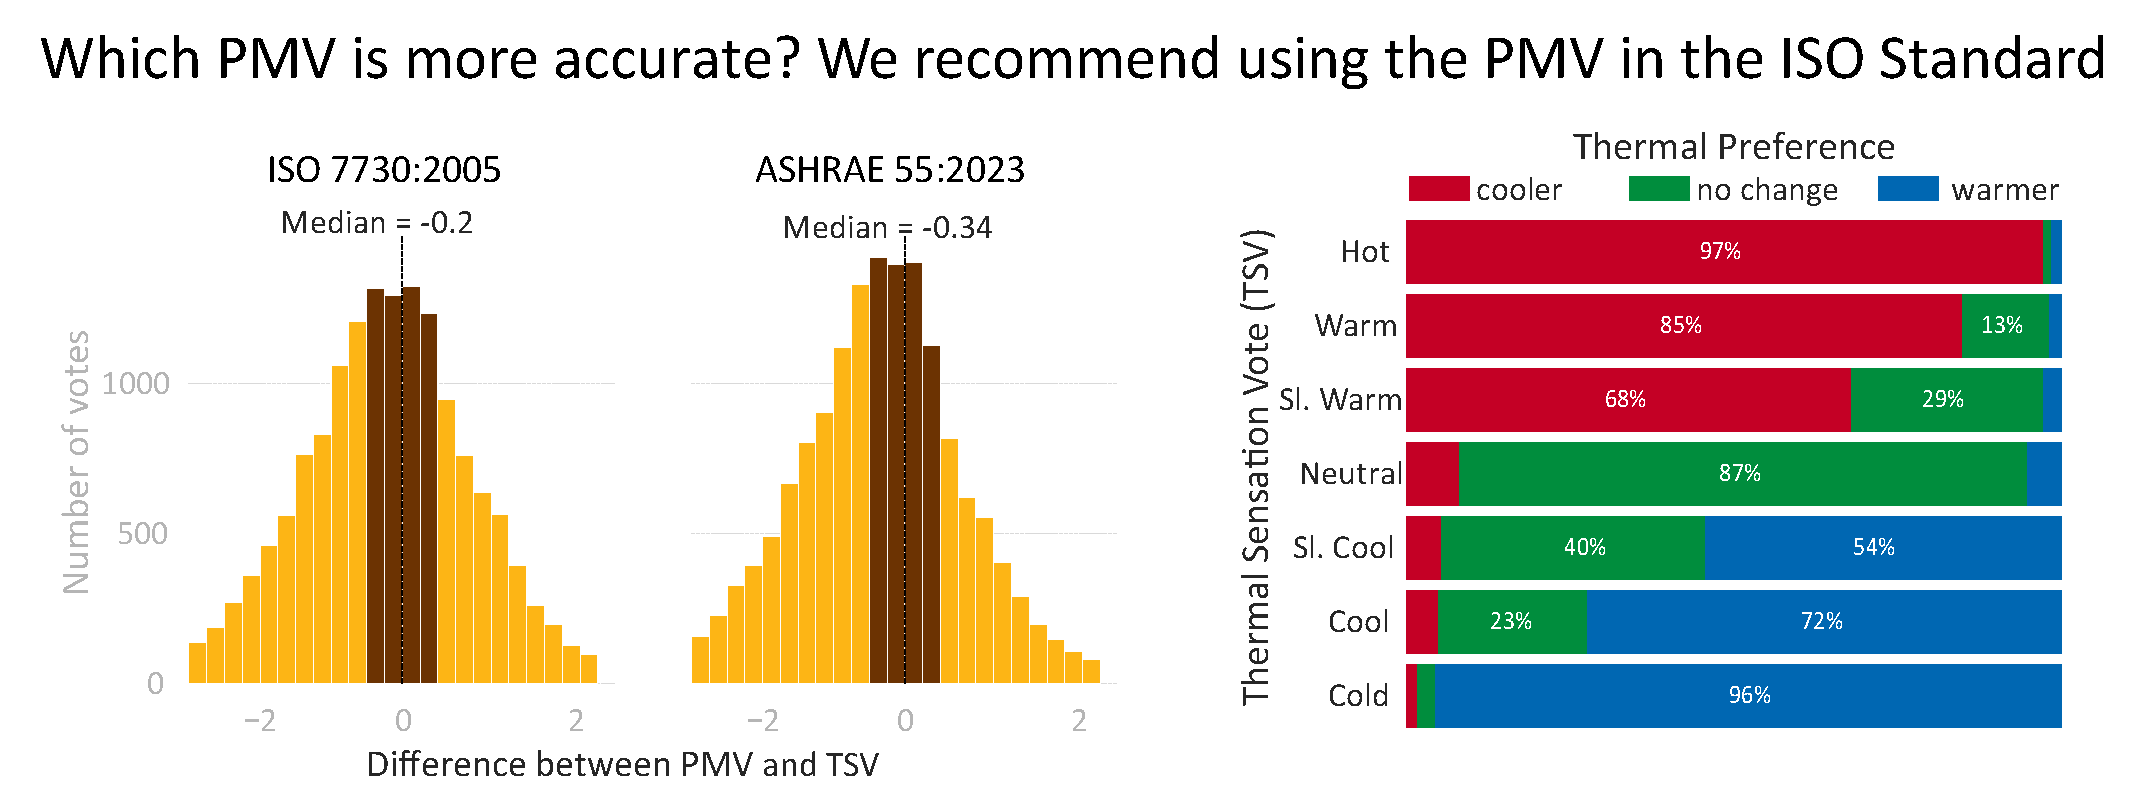
\includegraphics[width=\linewidth]{figures/graphical_abstract}
    \end{graphicalabstract}

    % Research highlights
    \begin{highlights}
        \item We compared the accuracy of the \ac{pmv} models in \gls{7730} and \gls{55}.
        \item Both models have low and similar prediction accuracy ($\approx$\qty{34}{\percent}).
        \item The \ac{pmv-ce} has a higher bias than \ac{pmv} in predicting thermal sensation.
        \item We recommend limiting the applicability range of the models to $\mid$\ac{pmv}$\mid \leq 0.5$.
        \item It is misleading to classify slightly warm/cool individuals as thermally comfortable.
    \end{highlights}

    \begin{keyword}
        Thermal comfort model \sep Predicted Mean Vote \sep Thermal comfort \sep Thermal sensation \sep Thermal preference
    \end{keyword}

\end{frontmatter}
